\chapter{Supplementary materials for \autoref{chap:CMZ}}
\section{Materials and methods}
\subsection{Zebrafish husbandry}
Zebrafish husbandry was performed as described in \autoref{ssec:husbandry}.
\subsection{PCNA Immunohistochemistry}
Anti-PCNA immunohistochemistry was performed as described in \autoref{ssec:PCNA}.
\subsection{Thymidine analogue histochemistry}
\label{ssec:CMZEdU}
Both cumulative thymidine analogue histochemistry presented in \autoref{ssec:CMZcumedu}, as well as the pulse-chase histochemistry used for the study of neural fate in \autoref{sec:neuralfate} were performed by the methods described in \autoref{ssec:SMMEcumedu} and \autoref{ssec:SMMEwholeretina}, respectively, except that the data from the whole retinal labelling experiment derives from 14\si{micro}{metre} transverse and coronal cryosections (n=3-6 animals per axis, per age). 

\subsection{Lineage tracing immunohistochemistry}
\label{ssec:CMZlintrace}
Embryos from wild-type AB crosses (staining groups 2 and 3) and \textit{Tg(Isl2b:GFP)} crosses (staining group 1). The \textit{Tg(Isl2b:GFP)} line was the kind gift of the late Dr. Chi-Bin Chien. Embryos were collected and reared as described in \autoref{ssec:husbandry}. Embryos were divided into three groups, to be pulsed with EdU at 3, 23, and 90 dpf and sacrificed after a 7 day chase period. In 3 and 23dpf larvae, animals were pulsed by allowing them to swim freely in a 10mM EdU solution for 2 hours. In 90dpf animals, 10\si{micro}{liters} of 10mM EdU was injected intraperitoneally. After 7 days, animals were sacrificed and coronal cryosections were obtained as described in \autoref{ssec:PCNA}. These cryosections were divided into staining groups according to their genetic origin, as mentioned above.

Cryosections from all staining groups were allowed to dry briefly at room temperature (RT), before rehydration in PBS for 30 minutes at RT.  Subsequently, sections were blocked in 0.2\% Triton X-100 + 2\% goat serum in PBS for 30 minutes at RT. Primary antibody incubations were as follows for each numbered staining group:

\begin{enumerate}
    \item Covance rabbit anti-Pax6 primary antibody diluted 1:200 in blocking solution incubated at 4\degree C overnight.
    \item Chemicon mouse anti-GS primary antibody diluted 1:500 in blocking solution at 4\degree C overnight.
    \item ZIRC mouse anti-Zpr1 primary antibody diluted 1:400 in blocking solution at 4\degree C overnight.
\end{enumerate}

After these overnight incubations, primary antibodies were removed and all sections were rinsed five times in PDT (PBS + 1\% DMSO + 0.1\% Tween-20). Secondary antibody incubations were as follows for each numbered staining group:

\begin{enumerate}
    \item Goat anti-rabbit Cy3-conjugated 2º antibody diluted 1:100 in blocking solution at 37°C for 2 hr.
    \item Goat anti-mouse Cy2-conjugated 2º antibody diluted 1:100 in blocking solution at 37°C for 2 hr.
    \item Goat anti-mouse Cy2-conjugated 2º antibody diluted 1:100 in blocking solution at 37°C for 2 hr.
\end{enumerate}

Staining group 2 was subsequently incubated with Santa Cruz rabbit anti-PKC$\beta$ 1º antibody diluted 1:100 in blocking solution at 4°C overnight. The next day, this second primary antibody was removed, and the group sections were rinsed in PDT as above. A further goat anti-mouse Cy2-conjugated 2º antibody diluted 1:100 in blocking sol’n was applied at 37°C for 2 hr.

After each staining group's final secondary antibody was removed, slides were rinsed 3x in PDT, then stained for EdU with an Alexa 647 azide. After another three PDT rinses, 100 ug/mL Hoechst 33258 was applied for 15 minutes at RT. Five PDT rinses, after which all slides were mounted, slipped, and sealed.

\subsection{4C4 immunohistochemistry}
\label{ssec:CMZ4C4histo}
The 4C4 antibody was a generous gift of Dr. Pamela Raymond. It has been empirically determined to mark microglia \cite{Becker2001}. It was used according to the methods described above with a Cy2 secondary antibody.

\subsection{Confocal micrograph acquisition and processing}
All confocal micrographs presented in \autoref{chap:CMZ} were acquired on a Leica TCS SP5 II microscope, operated using the LAS AF microscopy software (Leica). Data was assessed by using Bitplane Imaris software (v.). Specifically, the Imaris watershed segmentation algorithm was applied to the nuclear counterstain channel to segment cellular nuclei. Colocalisation of particular markers (ie. PCNA, EdU, or lineage markers) was assessed by thresholding signal from these channels with the segmented nuclear volumes to produce a subpopulation of colabelled nuclei. The segmented Imaris scenes and the associated settings are available in the thesis \hyperref[archive]{HDD archive}.

\subsection{Retinal measurements}
\label{ssec:CMZretmeas}
The developmental morphology study presented in \autoref{morphology} was conducted by using the LAS AF software measurement tools on transmitted light data collected in the process of conducting the confocal survey presented in \autoref{CMZoverall}. Each measurement point is, therefore, likewise the average of the value three central coronal cryosections. Retinal thickness was the linear thickness of the entire cellular retina and its plexiform layers at the center of the section, and the layer thicknesses reflect segments along this line, with the addition of RPE thickness. RPE length was measured in approximating segments from the dorsal to the ventral extrema. Lens diameter was measured in any sections which retained the lens; this was rare at older ages, when the lens sections tend to separate readily as soon as the cryosection is rehydrated. Optic nerve diameter was measured at its thickest point.

\subsection{Estimation of overall CMZ population and retinal volume}
\label{ssec:CMZpopvolest}
The overall CMZ population estimates were derived by the calculations presented in \autoref{sec:lenspopest}. The volume of the cellular retina was crudely estimated by subtracting the volume of two spheres. The circumference of the outer sphere is given by the RPE length plus the diameter of the lens. The radius of the inner sphere is the half total thickness of the cellular retina subtracted from radius of the outer sphere\footnote{Halving serves as crude compensation for the lack of cellular retina on the lens' part of the sphere, as well as the thinning of the cellular retina toward the periphery}. The difference in volume between the two spheres is calculated; four-fifths this value is taken as the volume estimate in order to partially compensate for the flattening of the eye at older ages.

\subsection{Monte Carlo estimation of CMZ population and retinal volume rates of change}
\label{ssec:MCrates}
In order to estimate the mean daily rate of change of the CMZ population and retinal volume estimates, we performed to Monte Carlo difference operations between samples drawn from the estimated LogNormal distributions at subsequent timepoints. This allows us to empirically estimate the uncertainty on these rates, as the difference between two T-distributions is not, itself, T-distributed.


\subsection{Evidence estimation by Empirical Bayes linear regression}
\label{ssec:CMZEmpBayes}
Evidence comparisons presented without estimated standard deviations ($\sigma$) of significance are produced by the \hyperref[ssec:EmpiricalBayes]{Empirical Bayes} method of linear regression, as presented in Bishop's standard machine learning textbook \cite{Bishop2006}. Calculations were performed using the Julia package \path{BayesianLinearRegression.jl}, which implements Bishop's algorithm in a high performance manner. 


% \autoref{EBtable} summarizes the \autoref{chap:CMZ} tables and figures which use this technique, along with links to model documentation and the code used to produce the table orfigure.

% \begin{table}[!ht]
%     \caption{Empirical Bayes estimates: models and code}
%     \begin{tabular}{|l|l|l|l|l|l|l|} 
%         \hline
%         {\bf Table/Figure} & {\bf Model} & {\bf Code} \\ \hline \hline

%     \end{tabular}
%     \label{EBtable}
% \end{table}

\subsection{Evidence estimation by Galilean Monte Carlo nested sampling}
\label{ssec:GMCev}

Evidence comparisons presented with estimated standard deviations ($\sigma$) of significance are produced by converging ensembles of \hyperref[GMC]{Galilean Monte Carlo} sample chains, which collectively constitute a sample from the posterior in rigorous detailed balance \cite{Skilling2019}. The \hyperref{BayesEpistemology}[Bayesian evidence], or marginal probability of the model over the posterior sample is calculated by the \hyperref{Nested}[nested sampling algorithm] \cite{Skilling2006}. Calculations were performed by the use of the Julia packages \path{GMC_NS.jl} and \path{CMZNicheSims.jl}, written for this thesis and presented in \autoref{chap:GMC} and \autoref{chap:CNS}, respectively. Maximum a posteriori outputs are calculated from the most likely model parameterisation sampled during this process.

% \autoref{GMCtable} summarizes the \autoref{chap:CMZ} figures which use these techniques, along with links to model documentation and the code used to produce the figures.

% \begin{table}[!ht]
%     \caption{Galilean Monte Carlo estimates: models and code}
%     \begin{tabular}{|l|l|l|l|l|l|l|} 
%         \hline
%         {\bf Table/Figure} & {\bf Model} & {\bf Code} \\ \hline \hline
%         \autoref{PZRtable} & \hyperref[NormalModels]{Normal \& LogNormal} & \autoref{ssec:a10nvln} \\ \hline
%     \end{tabular}
%     \label{GMCtable}
% \end{table}

\subsection{Estimation of posterior distributions of phase model parameters}
\label{ssec:GMCkde}
Posterior distributions presented in \autoref{phasemarginals} and \autoref{dvmarginals} were produced by Kernel Density Estimation (KDE) \cite[p. 122]{Bishop2006}. The KDE algorithm used was the implementation available in the Julia Robotics library \path{KernelDensityEstimate.jl}, described by Sudderth et al. \cite{Sudderth2010}. Briefly, this uses multiscale nonmparametric Gibbs sampling of supplied weighted ``point clouds'' to generate the kernel density estimate. Chains from \path{GMC_NS.jl} were used in this context by weighting the points in parameter space by their estimated evidence. It is important to note that, for this thesis, \path{GMC_NS.jl} was configured to prioritise the accuracy of evidence estimates over these posterior estimates; as a consequence, samples from around the maximum a posteriori have little weight in the KDE estimates presented herein \cite{Higson2018}. Alternatives to this scheme are possible; one such algorithm is described by Higson et al. \cite{Higson2019}

\section{Supplementary Figures}

\begin{figure}[!h]
    \makebox[\textwidth][c]{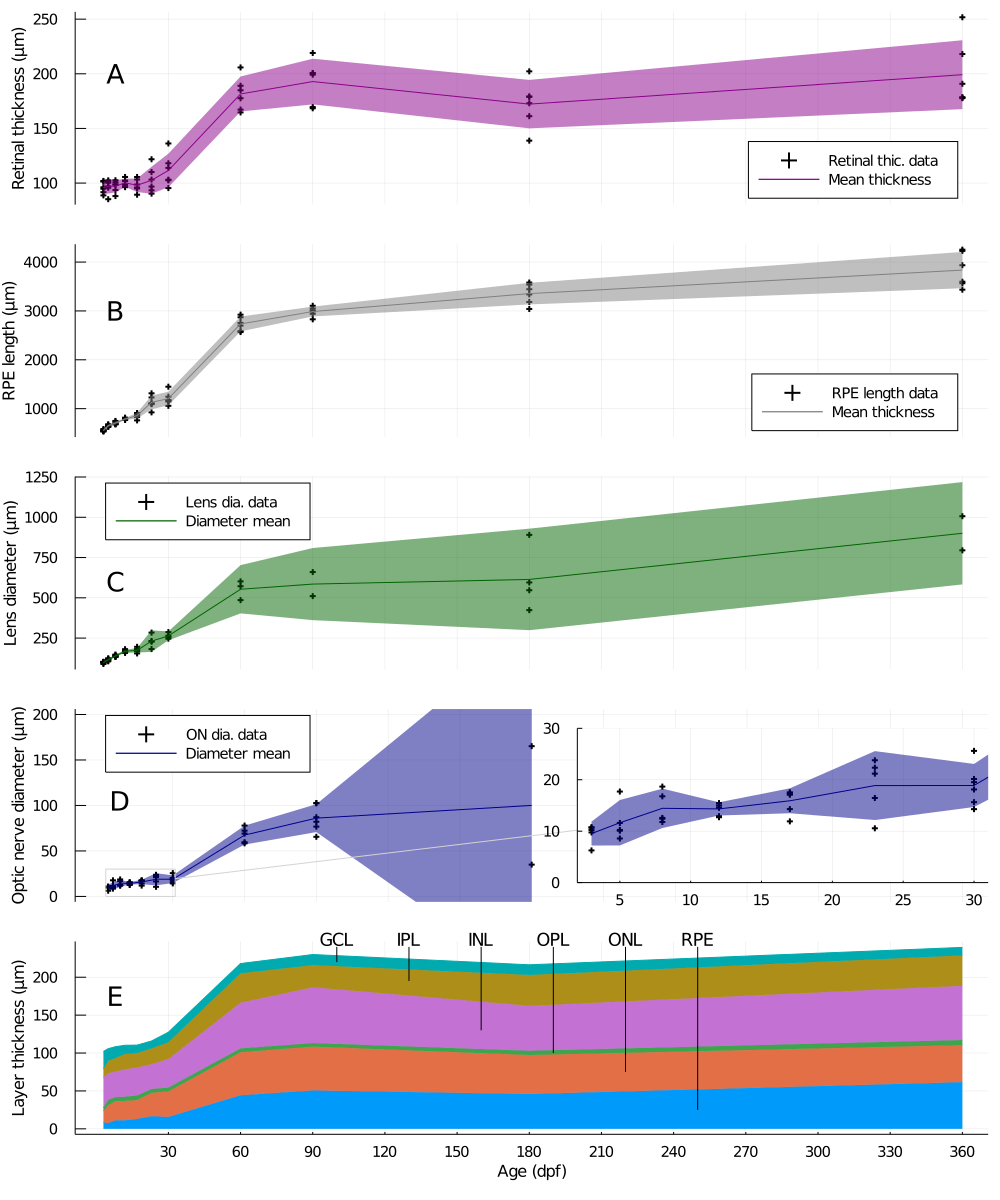
\includegraphics[width=1.2\textwidth]{cmz/morphology.png}}    
    \caption{{\bf Developmental progression of naso-temporal population asymmetry in the CMZ.}}
    \label{morphology}
\end{figure}

\begin{figure}[!h]
    \makebox[\textwidth][c]{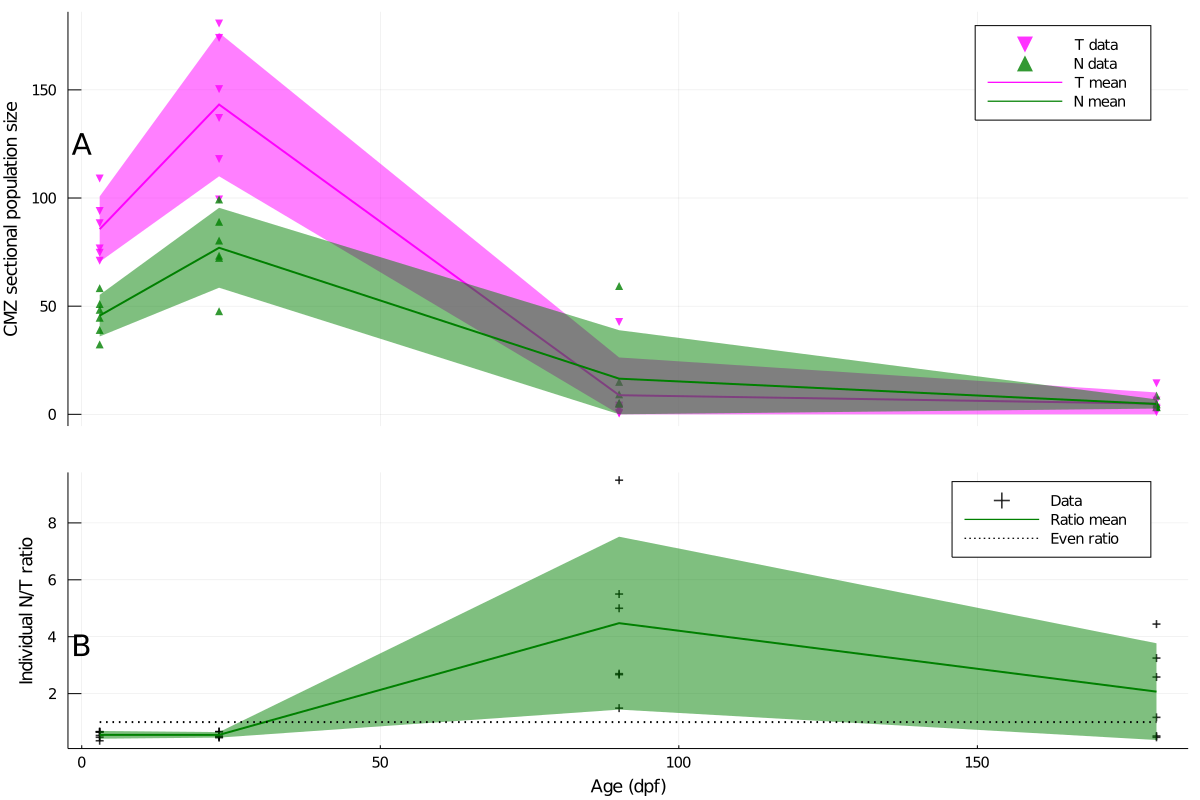
\includegraphics[width=1.2\textwidth]{cmz/NTontology.png}}    
    \caption{{\bf Developmental progression of naso-temporal population asymmetry in the CMZ.}}
    Marginal posterior distribution of mean nasal (N) and temporal (T) population size in 14$\mu$m transverse cryosections (panel A) or intra-individual N/T count asymmetry ratio (panel B), $\pm 95\%$ credible interval, n=6 animals per age. Data points represent mean counts from three central sections of an experimental animal's eye. 
    \label{NTontology}
\end{figure}


\begin{figure}[!h]
    \makebox[\textwidth][c]{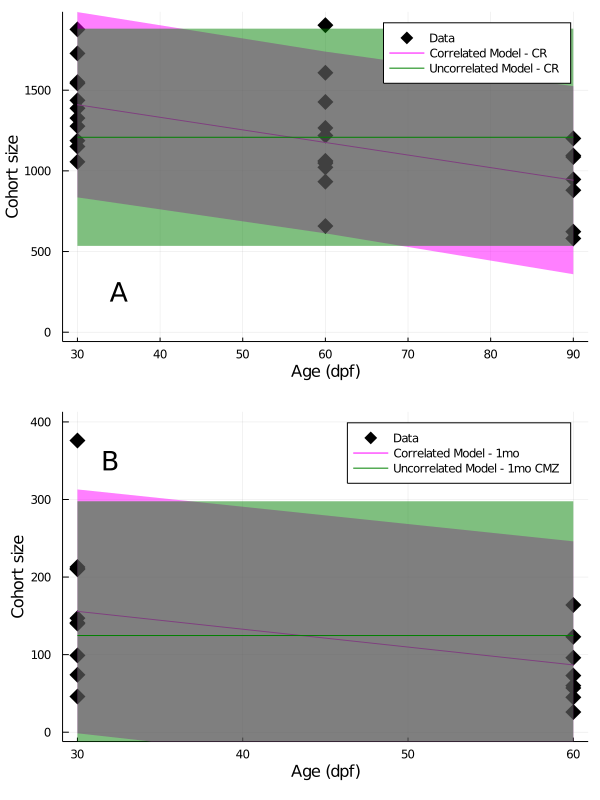
\includegraphics[width=.7\textwidth]{cmz/a27linreg.png}}    
    \caption{{\bf Linear regressions of temporally correlated and uncorrelated models of central retinal and 30dpf CMZ-contributed cohorts}}
    \label{a27linreg}
\end{figure}


\begin{figure}[!h]
    \makebox[\textwidth][c]{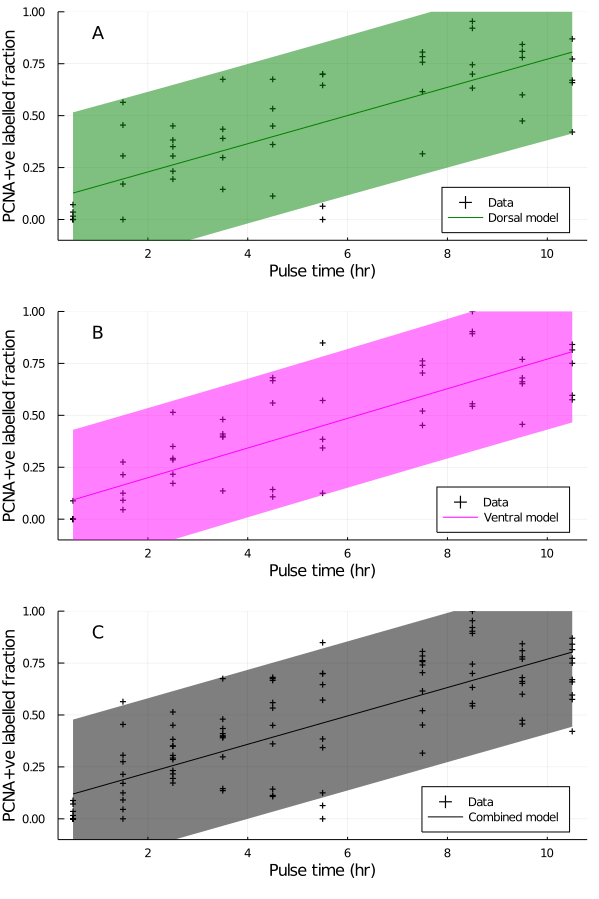
\includegraphics[width=.7\textwidth]{cmz/3ddvlinreg.png}}    
    \caption{{\bf Linear regressions performed on cumulative labelling data from dorsal, ventral, and combined CMZ sectional populations}}
    \label{cumEdUlinreg}
\end{figure}

\begin{figure}[!h]
    \makebox[\textwidth][c]{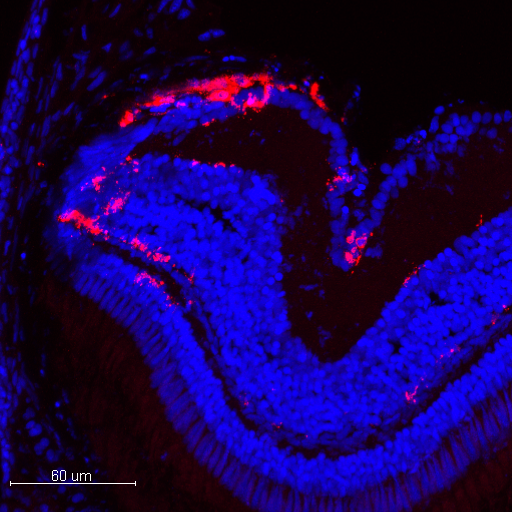
\includegraphics[width=.6\textwidth]{cmz/4C4 distribution.png}}    
    \caption{{\bf 4C4+ microglia are associated with the CMZ}}
    Representative maximum intensity projection from confocal micrographs of 14\si{\micro\metre} coronal cryosections through 90dpf zebrafish eyes.
    
    Blue: Hoechst 33258 nuclear counterstain. Red: Microglia labelled with 4C4 antibody. Note extensive presence of 4C4+ microglia around the peripheral CMZ.
    \label{4C4micrograph}
\end{figure}

\FloatBarrier

\section{Evidence calculations for models of layer and lineage contribution}
\FloatBarrier

\begin{table}[!ht]
    \caption{Evidence for Normal vs. Log-Normal models of layer and lineage contribution}
    \begin{tabular}{|l|l|l|l|l|l|l|} 
        \hline
        {\bf Layer} & {\bf Marker} & {\bf Cell type} & {\bf $\mathcal{N}$ logZ} & {\bf Log-$\mathcal{N}$ logZ} & {\bf logZR} & {\bf $\sigma$ sign.}\\ \hline \hline
        GCL & Cohort & All GCL cells & -92.81 ± 0.56 & {\bf-63.93 ± 0.19} & 28.88 ± 0.6 & 48.5\\ \hline \hline
        GCL & Isl2b & RGC & -56.3 ± 0.76 & {\bf -46.91 ± 0.35} & 9.38 ± 0.84 & 11.2\\ \hline
        GCL & Pax6 & Displaced am. & -110.7 ± 1.2 & {\bf -35.39 ± 0.34} & 75.3 ± 1.2 & 62.1\\ \hline
        GCL & Isl2b/Pax6 & RGC subtype & -16.38 ± 0.18 & {\bf -3.25 ± 0.6} & 13.13 ± 0.63 & 20.9\\ \hline \hline
        INL & Cohort & All INL cells & {\bf -84.56 ± 0.91} & -286.89 ± 0.68 & -202.3 ± 1.1 & 178.3\\ \hline \hline
        INL & Pax6 & Amacrine cell & {\bf -13.99 ± 0.24} & -18.5 ± 0.25 & -4.52 ± 0.35 & 12.9\\ \hline
        INL & PKC$\beta$ & Bipolar cell & -13.66 ± 0.16 & {\bf 8.68 ± 0.44} & 22.34 ± 0.47 & 47.7\\ \hline
        INL & GS & M\"{u}ller glia & -12.36 ± 0.23 & {\bf 14.18 ± 0.48} & 26.54 ± 0.53 & 50.3\\ \hline
        INL & HM & Horizontal cell & -16.44 ± 0.27 & {\bf 9.15 ± 0.37} & 25.59 ± 0.46 & 55.6\\ \hline \hline
        ONL & Cohort & All ONL cells & {\bf -128.68 ± 1.0} & -171.66 ± 0.63 & -43.0 ± 1.2 & 36.5\\ \hline \hline
        ONL & Zpr1 & Double cones & {\bf -42.25 ± 0.72} & -54.25 ± 0.37 & -11.99 ± 0.81 & 14.9\\ \hline
    \end{tabular}
   
    \begin{flushleft}logZ: logarithm of p(D), the marginal likelihood of the data, or model evidence.  Largest evidence values bolded. logZR: evidence ratio; positive values in favour of Log-$\mathcal{N}$ model.
    \end{flushleft}
    \label{lineage_nlnev}
\end{table}

\begin{table}[!ht]
    \caption{Evidence for combined vs. split models of layer and lineage contribution across the dorso-ventral axis}
    \begin{tabular}{|l|l|l|l|l|l|l|} 
        \hline
        {\bf Layer} & {\bf Marker} & {\bf Cell type} & {\bf Combined D-V logZ} & {\bf Split D-V logZ} & {\bf logZR} & {\bf $\sigma$ sign.}\\ \hline \hline
        GCL & Cohort & All GCL cells & {\bf -53.473 ± 0.055} & -184.34 ± 0.13 & 130.86 ± 0.14 & 911.5\\ \hline \hline
        GCL & Isl2b & RGC & {\bf -54.58 ± 0.9} & -67.72 ± 0.94 & 13.1 ± 1.3 & 10.1\\ \hline
        GCL & Pax6 & Displaced am. & {\bf -31.09 ± 0.12} & -46.41 ± 0.3 & 15.32 ± 0.33 & 46.9\\ \hline
        GCL & Isl2b/Pax6 & RGC subtype & {\bf -43.76 ± 0.76} & -109.0 ± 1.3 & 65.3 ± 1.5 & 43.3\\ \hline \hline
        INL & Cohort & All INL cells & {\bf -131.4 ± 1.4} & -184.4 ± 1.6 & 52.9 ± 2.1 & 25.0\\ \hline \hline
        INL & Pax6 & Amacrine cell & {\bf -15.8 ± 0.024} & -52.42 ± 0.69 & 36.62 ± 0.69 & 53.3\\ \hline
        INL & PKC$\beta$ & Bipolar cell & {\bf -3.86 ± 0.2} & -19.81 ± 0.23 & 15.96 ± 0.31 & 51.9\\ \hline
        INL & GS & M\"{u}ller glia & {\bf 15.78 ± 0.25} & 28.03 ± 0.41 & -12.24 ± 0.48 & -25.6\\ \hline
        INL & HM & Horizontal cell & {\bf 10.79 ± 0.41} & -3.65 ± 0.19 & 14.45 ± 0.45 & 32.2\\ \hline \hline
        ONL & Cohort & All ONL cells & {\bf -79.87 ± 0.97} & -158.2 ± 1.3 & 78.3 ± 1.6 & 48.5\\ \hline \hline
        ONL & Zpr1 & Double cones & {\bf -54.66 ± 0.92} & -64.27 ± 0.87 & 9.6 ± 1.3 & 7.6\\ \hline
    \end{tabular}
\begin{flushleft}logZ: logarithm of p(D), the marginal likelihood of the data, or model evidence.  Largest evidence values bolded. logZR: evidence ratio; positive values in favour of combined model.
\end{flushleft}
\label{lineage_dvev}
\end{table}

\section{Likelihood ratio calculations for Normal and Log-Normal models of layer and lineage contribution}

\begin{table}[!ht]
    \begin{tabular}{|l|l|l|l|l|l|l|} 
        \hline
        {\bf Layer} & {\bf Marker} & {\bf Cell type} & {\bf $\mathcal{N}$ MLE} & {\bf Log-$\mathcal{N}$ MLE} & {\bf lhR}\\ \hline \hline
        GCL & Cohort & All GCL cells & 54.194 & {\bf 55.835} & 1.642\\ \hline
        GCL & Isl2b & RGC & 14.439 & {\bf 19.106} & 4.667\\ \hline
        GCL & Pax6 & Displaced am. &  8.287 & {\bf 11.158} & 2.871\\ \hline
        GCL & Isl2b/Pax6 & RGC subtype & 20.292 & {\bf 28.139} & 7.847\\ \hline
        INL & Cohort & All INL cells & 44.942 & {\bf 45.179} & 0.237\\ \hline
        INL & Pax6 & Amacrine cell & {\bf 23.808} & 23.178 & -0.63\\ \hline
        INL & PKC$\beta$ & Bipolar cell & {\bf 27.243} & 26.119 & -1.124\\ \hline
        INL & GS & M\"{u}ller glia & 30.847 & {\bf 31.818} & 0.97\\ \hline
        INL & HM & Horizontal cell & 27.65 & {\bf 29.431} & 1.78\\ \hline
        ONL & Cohort & All ONL cells & 41.488 & {\bf 43.195} & 1.706\\ \hline
        ONL & Zpr1 & Double cones & 13.256 & {\bf 18.483} & 5.227\\ \hline
    \end{tabular}
   
    \begin{flushleft}logZ: logarithm of p(D), the marginal likelihood of the data, or model evidence.  Largest evidence values bolded. logZR: evidence ratio; positive values in favour of stable model.
    \end{flushleft}
    \label{lineage_lhratio}
\end{table}


